% Options for packages loaded elsewhere
\PassOptionsToPackage{unicode}{hyperref}
\PassOptionsToPackage{hyphens}{url}
%
\documentclass[
]{book}
\usepackage{amsmath,amssymb}
\usepackage{iftex}
\ifPDFTeX
  \usepackage[T1]{fontenc}
  \usepackage[utf8]{inputenc}
  \usepackage{textcomp} % provide euro and other symbols
\else % if luatex or xetex
  \usepackage{unicode-math} % this also loads fontspec
  \defaultfontfeatures{Scale=MatchLowercase}
  \defaultfontfeatures[\rmfamily]{Ligatures=TeX,Scale=1}
\fi
\usepackage{lmodern}
\ifPDFTeX\else
  % xetex/luatex font selection
\fi
% Use upquote if available, for straight quotes in verbatim environments
\IfFileExists{upquote.sty}{\usepackage{upquote}}{}
\IfFileExists{microtype.sty}{% use microtype if available
  \usepackage[]{microtype}
  \UseMicrotypeSet[protrusion]{basicmath} % disable protrusion for tt fonts
}{}
\makeatletter
\@ifundefined{KOMAClassName}{% if non-KOMA class
  \IfFileExists{parskip.sty}{%
    \usepackage{parskip}
  }{% else
    \setlength{\parindent}{0pt}
    \setlength{\parskip}{6pt plus 2pt minus 1pt}}
}{% if KOMA class
  \KOMAoptions{parskip=half}}
\makeatother
\usepackage{xcolor}
\usepackage{color}
\usepackage{fancyvrb}
\newcommand{\VerbBar}{|}
\newcommand{\VERB}{\Verb[commandchars=\\\{\}]}
\DefineVerbatimEnvironment{Highlighting}{Verbatim}{commandchars=\\\{\}}
% Add ',fontsize=\small' for more characters per line
\usepackage{framed}
\definecolor{shadecolor}{RGB}{248,248,248}
\newenvironment{Shaded}{\begin{snugshade}}{\end{snugshade}}
\newcommand{\AlertTok}[1]{\textcolor[rgb]{0.94,0.16,0.16}{#1}}
\newcommand{\AnnotationTok}[1]{\textcolor[rgb]{0.56,0.35,0.01}{\textbf{\textit{#1}}}}
\newcommand{\AttributeTok}[1]{\textcolor[rgb]{0.13,0.29,0.53}{#1}}
\newcommand{\BaseNTok}[1]{\textcolor[rgb]{0.00,0.00,0.81}{#1}}
\newcommand{\BuiltInTok}[1]{#1}
\newcommand{\CharTok}[1]{\textcolor[rgb]{0.31,0.60,0.02}{#1}}
\newcommand{\CommentTok}[1]{\textcolor[rgb]{0.56,0.35,0.01}{\textit{#1}}}
\newcommand{\CommentVarTok}[1]{\textcolor[rgb]{0.56,0.35,0.01}{\textbf{\textit{#1}}}}
\newcommand{\ConstantTok}[1]{\textcolor[rgb]{0.56,0.35,0.01}{#1}}
\newcommand{\ControlFlowTok}[1]{\textcolor[rgb]{0.13,0.29,0.53}{\textbf{#1}}}
\newcommand{\DataTypeTok}[1]{\textcolor[rgb]{0.13,0.29,0.53}{#1}}
\newcommand{\DecValTok}[1]{\textcolor[rgb]{0.00,0.00,0.81}{#1}}
\newcommand{\DocumentationTok}[1]{\textcolor[rgb]{0.56,0.35,0.01}{\textbf{\textit{#1}}}}
\newcommand{\ErrorTok}[1]{\textcolor[rgb]{0.64,0.00,0.00}{\textbf{#1}}}
\newcommand{\ExtensionTok}[1]{#1}
\newcommand{\FloatTok}[1]{\textcolor[rgb]{0.00,0.00,0.81}{#1}}
\newcommand{\FunctionTok}[1]{\textcolor[rgb]{0.13,0.29,0.53}{\textbf{#1}}}
\newcommand{\ImportTok}[1]{#1}
\newcommand{\InformationTok}[1]{\textcolor[rgb]{0.56,0.35,0.01}{\textbf{\textit{#1}}}}
\newcommand{\KeywordTok}[1]{\textcolor[rgb]{0.13,0.29,0.53}{\textbf{#1}}}
\newcommand{\NormalTok}[1]{#1}
\newcommand{\OperatorTok}[1]{\textcolor[rgb]{0.81,0.36,0.00}{\textbf{#1}}}
\newcommand{\OtherTok}[1]{\textcolor[rgb]{0.56,0.35,0.01}{#1}}
\newcommand{\PreprocessorTok}[1]{\textcolor[rgb]{0.56,0.35,0.01}{\textit{#1}}}
\newcommand{\RegionMarkerTok}[1]{#1}
\newcommand{\SpecialCharTok}[1]{\textcolor[rgb]{0.81,0.36,0.00}{\textbf{#1}}}
\newcommand{\SpecialStringTok}[1]{\textcolor[rgb]{0.31,0.60,0.02}{#1}}
\newcommand{\StringTok}[1]{\textcolor[rgb]{0.31,0.60,0.02}{#1}}
\newcommand{\VariableTok}[1]{\textcolor[rgb]{0.00,0.00,0.00}{#1}}
\newcommand{\VerbatimStringTok}[1]{\textcolor[rgb]{0.31,0.60,0.02}{#1}}
\newcommand{\WarningTok}[1]{\textcolor[rgb]{0.56,0.35,0.01}{\textbf{\textit{#1}}}}
\usepackage{longtable,booktabs,array}
\usepackage{calc} % for calculating minipage widths
% Correct order of tables after \paragraph or \subparagraph
\usepackage{etoolbox}
\makeatletter
\patchcmd\longtable{\par}{\if@noskipsec\mbox{}\fi\par}{}{}
\makeatother
% Allow footnotes in longtable head/foot
\IfFileExists{footnotehyper.sty}{\usepackage{footnotehyper}}{\usepackage{footnote}}
\makesavenoteenv{longtable}
\usepackage{graphicx}
\makeatletter
\def\maxwidth{\ifdim\Gin@nat@width>\linewidth\linewidth\else\Gin@nat@width\fi}
\def\maxheight{\ifdim\Gin@nat@height>\textheight\textheight\else\Gin@nat@height\fi}
\makeatother
% Scale images if necessary, so that they will not overflow the page
% margins by default, and it is still possible to overwrite the defaults
% using explicit options in \includegraphics[width, height, ...]{}
\setkeys{Gin}{width=\maxwidth,height=\maxheight,keepaspectratio}
% Set default figure placement to htbp
\makeatletter
\def\fps@figure{htbp}
\makeatother
\setlength{\emergencystretch}{3em} % prevent overfull lines
\providecommand{\tightlist}{%
  \setlength{\itemsep}{0pt}\setlength{\parskip}{0pt}}
\setcounter{secnumdepth}{5}
\usepackage{booktabs}
\ifLuaTeX
  \usepackage{selnolig}  % disable illegal ligatures
\fi
\usepackage[]{natbib}
\bibliographystyle{plainnat}
\usepackage{bookmark}
\IfFileExists{xurl.sty}{\usepackage{xurl}}{} % add URL line breaks if available
\urlstyle{same}
\hypersetup{
  pdftitle={Guide R},
  pdfauthor={Prof.~Audrey Bürki, Samuel Arthers, Mégane Bollenrücher},
  hidelinks,
  pdfcreator={LaTeX via pandoc}}

\title{Guide R}
\author{Prof.~Audrey Bürki, Samuel Arthers, Mégane Bollenrücher}
\date{2024-09-22}

\begin{document}
\maketitle

{
\setcounter{tocdepth}{1}
\tableofcontents
}
Merci de prendre note que ce bookdown est en cours de rédaction.

\chapter{Introduction}\label{introduction}

Ceci est le guide R que nous proposons pour vous accompagner durant le cours de Statistiques I.

\chapter{Installation et environnement R et Rstudio}\label{installation-et-environnement-r-et-rstudio}

\section{Présentation des logiciels}\label{pruxe9sentation-des-logiciels}

R est un langage de programmation adapté au traitement de données et à l'analyse statistique.

Pour programmer en langage R, il est nécessaire d'installer deux outils essentiels:

\begin{enumerate}
\def\labelenumi{\arabic{enumi}.}
\tightlist
\item
  Le \textbf{logiciel R} permet de traduire du texte sous forme de code R en binaire qui est le langage interne du processeur de l'ordinateur.
\item
  Le \textbf{logiciel RStudio} permet de faciliter l'utilisation du logiciel R en donnant l'accès à une interface utilisateur.
\end{enumerate}

Il est possible de faire une analogie avec une voiture. Le logiciel R est le moteur et RStudio est le tableau de bord. Sans le tableau de bord, il n'est pas possible de controler le moteur.

\section{Installation}\label{installation}

\begin{enumerate}
\def\labelenumi{\arabic{enumi}.}
\tightlist
\item
  Installer R sur le site de R.

  \begin{enumerate}
  \def\labelenumii{\roman{enumii}.}
  \tightlist
  \item
    Choisir et télécharger la version de R selon votre système d'exploitation.

    \begin{itemize}
    \tightlist
    \item
      Pour windows : \url{https://cran.r-project.org/bin/windows/base/}
    \item
      Pour MAC : \url{https://cran.r-project.org/bin/macosx/}
    \item
      Pour Linux : \url{https://cran.r-project.org/index.html}
    \end{itemize}
  \item
    Installer le logiciel R sur votre ordinateur en exécutant le fichier téléchargé.
  \end{enumerate}
\item
  Installer RStudio sur le site suivant: \url{https://posit.co/download/rstudio-desktop/}
\end{enumerate}

Après avoir installé ces deux logiciels, vous aurez accès à deux nouvelles applications. Cependant, nous utiliserons uniquement RStudio pour programmer. Lorsque vous exécuterez votre code écrit sur RStudio, ce dernier fera automatiquement appel à R pour exécuter les codes.

\section{Environnement de travail}\label{environnement-de-travail}

Une fois que RStudio est lancé, une interface découpée en plusieurs zones se présente. Ces parties parties peuvent être redimensionnées, masquées ou maximisées selon vos préférences.

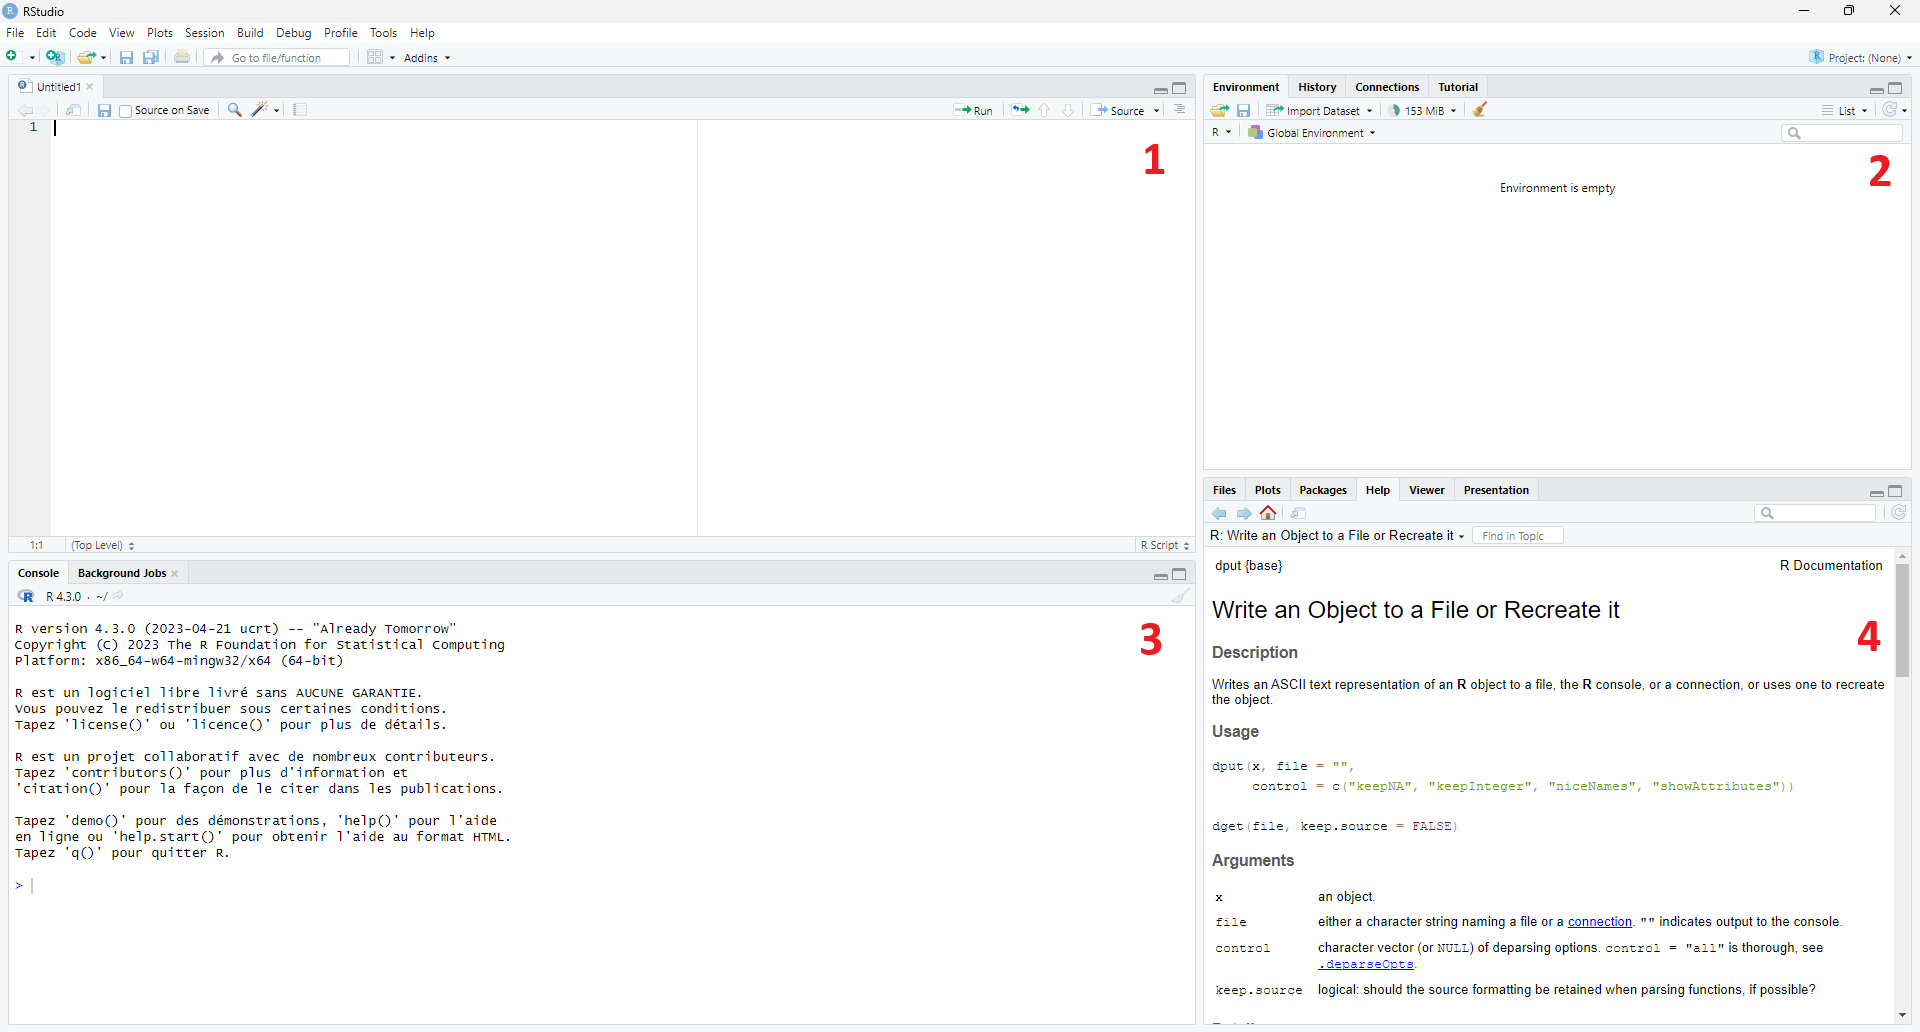
\includegraphics{images/environnement.png}
Chacune des quatre zones a sa propre utilité:

\begin{enumerate}
\def\labelenumi{\arabic{enumi}.}
\tightlist
\item
  Cette zone est dédiée aux fichiers sources. Ce volet permet d'écrire et de sauvegarder les lignes de code. Ce sera la partie la plus utilisée lors de la programmation.
\item
  Cette zone fournit des informations sur les objets, les variables et les données en mémoire sous l'onglet \texttt{Environment}.
\item
  La console est affichée en bas à gauche. Cette partie permet d'entrer et d'exécuter des instructions et voir les résultats s'afficher.
\item
  Cette zone permet de naviguer dans le répertoire de travail dans l'onglet \texttt{Files}, d'afficher les graphes réalisés dans l'onglet \texttt{Plots}, d'afficher les extensions/packages disponibles sous l'onglet \texttt{Packages} et également d'afficher l'aide (qui est très complète) sous l'onglet \texttt{Help}.
\end{enumerate}

\chapter{Objets et opérateurs}\label{objets-et-opuxe9rateurs}

\section{Objets dans R}\label{objets-dans-r}

Une variable permet de stocker une valeur ou un objet dans R. De cette façon, il sera possible d'accéder à la valeur ou à l'objet qui est stocké dans la variable.

\begin{Shaded}
\begin{Highlighting}[]
\CommentTok{\# Assignation de la valeur 3 à la variable "ma\_variable"}
\NormalTok{ma\_variable }\OtherTok{\textless{}{-}} \DecValTok{3}
\end{Highlighting}
\end{Shaded}

La ligne de code ci-dessus déclare une variable nommée ``ma\_variable'' et lui assigne la valeur de 3. L'exécution de ce code n'affiche pas de résultat dans la console, mais l'objet nommé ``ma\_variable'' est bien créée et stockée dans l'environnement.

Pour afficher le contenu de la variable, il suffit de taper le nom de celle-ci pour l'afficher dans la console.

\begin{Shaded}
\begin{Highlighting}[]
\CommentTok{\# Affichage du contenu de la variable "ma\_variable"}
\NormalTok{ma\_variable}
\end{Highlighting}
\end{Shaded}

\begin{verbatim}
## [1] 3
\end{verbatim}

De plus, il est également possible d'utiliser la fonction \texttt{print()} qui permet d'afficher la valeur ou l'objet de la variable sélectionnée.

\begin{Shaded}
\begin{Highlighting}[]
\CommentTok{\# Affichage du contenur de la variable "ma\_variable"}
\FunctionTok{print}\NormalTok{(ma\_variable)}
\end{Highlighting}
\end{Shaded}

\begin{verbatim}
## [1] 3
\end{verbatim}

En langage R, il existe différents types d'objets qui peuvent être assignés à des variables comme les scalaires, les vecteurs, les facteurs, les matrices et les bases de données. Ces objets sont présentés dans les points suivants.

\subsection{Scalaire}\label{scalaire}

Un scalaire permet de stocker un objet sous forme de valeur numérique, de chaîne de caractères ou de valeur logique.

\begin{Shaded}
\begin{Highlighting}[]
\CommentTok{\# Scalaire numerique}
\NormalTok{a }\OtherTok{\textless{}{-}} \DecValTok{3}
\NormalTok{a}
\end{Highlighting}
\end{Shaded}

\begin{verbatim}
## [1] 3
\end{verbatim}

Une chaîne de caractères est une suite de caractères qui doit être écrit entre guillemets ('' ``).

\begin{Shaded}
\begin{Highlighting}[]
\CommentTok{\# Scalaire sous forme d\textquotesingle{}une chaine de caractères}
\NormalTok{b }\OtherTok{\textless{}{-}} \StringTok{"Statistique"}
\NormalTok{b}
\end{Highlighting}
\end{Shaded}

\begin{verbatim}
## [1] "Statistique"
\end{verbatim}

Une valeur logique est une quantitée binaire (vrai ou faux). Ces variables s'écrivent \texttt{TRUE} et \texttt{FALSE}. Il est également possible d'utiliser \texttt{T} et \texttt{F} comme abréviations.

\begin{Shaded}
\begin{Highlighting}[]
\CommentTok{\# Scalaire logique}
\NormalTok{c }\OtherTok{\textless{}{-}} \ConstantTok{TRUE}
\NormalTok{c}
\end{Highlighting}
\end{Shaded}

\begin{verbatim}
## [1] TRUE
\end{verbatim}

\begin{Shaded}
\begin{Highlighting}[]
\NormalTok{d }\OtherTok{\textless{}{-}}\NormalTok{ F}
\NormalTok{d  }
\end{Highlighting}
\end{Shaded}

\begin{verbatim}
## [1] FALSE
\end{verbatim}

\subsection{Vecteur}\label{vecteur}

Un vecteur est un objet qui permet de stocker une liste ordonnée d'éléments. Les éléments d'un vecteur doivent être du même type.
Pour pouvoir stocker une information dans un seul objet, il faut utiliser la fonction \texttt{c()} qui permet de combiner les arguments de la fonction.

\begin{Shaded}
\begin{Highlighting}[]
\CommentTok{\# Vecteur numérique}
\NormalTok{a }\OtherTok{\textless{}{-}} \FunctionTok{c}\NormalTok{(}\DecValTok{1}\NormalTok{, }\DecValTok{2}\NormalTok{, }\DecValTok{3}\NormalTok{, }\DecValTok{4}\NormalTok{, }\DecValTok{5}\NormalTok{, }\DecValTok{6}\NormalTok{)}
\NormalTok{a}
\end{Highlighting}
\end{Shaded}

\begin{verbatim}
## [1] 1 2 3 4 5 6
\end{verbatim}

\begin{Shaded}
\begin{Highlighting}[]
\CommentTok{\# Vecteur sous forme d\textquotesingle{}une chaine de caractères}
\NormalTok{b }\OtherTok{\textless{}{-}} \FunctionTok{c}\NormalTok{(}\StringTok{"Un"}\NormalTok{, }\StringTok{"Deux"}\NormalTok{, }\StringTok{"Trois"}\NormalTok{, }\StringTok{"Quatre"}\NormalTok{, }\StringTok{"Cinq"}\NormalTok{, }\StringTok{"Six"}\NormalTok{)}
\NormalTok{b}
\end{Highlighting}
\end{Shaded}

\begin{verbatim}
## [1] "Un"     "Deux"   "Trois"  "Quatre" "Cinq"   "Six"
\end{verbatim}

\begin{Shaded}
\begin{Highlighting}[]
\CommentTok{\# Vecteur logique}
\NormalTok{c }\OtherTok{\textless{}{-}} \FunctionTok{c}\NormalTok{(}\ConstantTok{TRUE}\NormalTok{, }\ConstantTok{FALSE}\NormalTok{, }\ConstantTok{TRUE}\NormalTok{, }\ConstantTok{FALSE}\NormalTok{, }\ConstantTok{FALSE}\NormalTok{, }\ConstantTok{TRUE}\NormalTok{)}
\NormalTok{c}
\end{Highlighting}
\end{Shaded}

\begin{verbatim}
## [1]  TRUE FALSE  TRUE FALSE FALSE  TRUE
\end{verbatim}

Étant donné que le vecteur est un objet ordonné, il est possible d'accéder, remplacer ou modifier un ou plusieurs éléments par rapport à leur position dans l'objet. Il est nécessaire d'utiliser les crochets \texttt{{[}\ {]}} pour indiquer le ou les éléments à manipuler.

Pour accéder un seul élément du vecteur, il suffit d'écrire le nom de la variable suivi de crochets contenant la position de l'élément sélectionné.

\begin{Shaded}
\begin{Highlighting}[]
\CommentTok{\# Extraction d\textquotesingle{}un élément:}
\NormalTok{b[}\DecValTok{2}\NormalTok{]}
\end{Highlighting}
\end{Shaded}

\begin{verbatim}
## [1] "Deux"
\end{verbatim}

Il est possible d'accéder à plusieurs éléments en mettant un vecteur de position entre crochets.

\begin{Shaded}
\begin{Highlighting}[]
\CommentTok{\# Extraction de plusieurs éléments:}
\NormalTok{b[}\FunctionTok{c}\NormalTok{(}\DecValTok{2}\NormalTok{,}\DecValTok{3}\NormalTok{,}\DecValTok{5}\NormalTok{)]}
\end{Highlighting}
\end{Shaded}

\begin{verbatim}
## [1] "Deux"  "Trois" "Cinq"
\end{verbatim}

Il est aussi possible d'accéder à une série d'éléments à la suite en mettant le signe \texttt{:} entre les 2 positions désirées.

\begin{Shaded}
\begin{Highlighting}[]
\CommentTok{\# Extraction d\textquotesingle{}une série d\textquotesingle{}éléments:}
\NormalTok{b[}\DecValTok{2}\SpecialCharTok{:}\DecValTok{5}\NormalTok{]}
\end{Highlighting}
\end{Shaded}

\begin{verbatim}
## [1] "Deux"   "Trois"  "Quatre" "Cinq"
\end{verbatim}

Il est également possible d'accéder à certaines lignes en fonction de la valeur logique d'un vecteur ayant la même taille du vecteur sélectionné. Si la position est mise à \texttt{TRUE}, la valeur sera sélectionnée et dans le cas dans lequel la valeur est mise à \texttt{FALSE} la valeur ne sera pas retenue.

\begin{Shaded}
\begin{Highlighting}[]
\CommentTok{\# Extraction de plusieurs éléments en fontion de la valeur logique:}
\NormalTok{b[}\FunctionTok{c}\NormalTok{(}\ConstantTok{FALSE}\NormalTok{, }\ConstantTok{TRUE}\NormalTok{, }\ConstantTok{TRUE}\NormalTok{, }\ConstantTok{FALSE}\NormalTok{, }\ConstantTok{TRUE}\NormalTok{, }\ConstantTok{TRUE}\NormalTok{)]}
\end{Highlighting}
\end{Shaded}

\begin{verbatim}
## [1] "Deux"  "Trois" "Cinq"  "Six"
\end{verbatim}

\subsection{Facteur}\label{facteur}

Un facteur est un vecteur dont les éléments peuvent prendre que des valeurs prédéfinies. Un facteur dispose de l'argument \texttt{levels} qui permet de définir des catégories de valeurs. Le facteur est généralement utilisé pour stocker des variables catégorielles.

Pour commencer, il faut définir un vecteur qui peut être numérique, logique ou chaine de caractères. Le facteur est une variable nominale.

\begin{Shaded}
\begin{Highlighting}[]
\NormalTok{genre }\OtherTok{\textless{}{-}} \FunctionTok{c}\NormalTok{(}\StringTok{"Homme"}\NormalTok{, }\StringTok{"Femme"}\NormalTok{, }\StringTok{"Femme"}\NormalTok{, }\StringTok{"Femme"}\NormalTok{, }\StringTok{"Homme"}\NormalTok{)}
\NormalTok{genre}
\end{Highlighting}
\end{Shaded}

\begin{verbatim}
## [1] "Homme" "Femme" "Femme" "Femme" "Homme"
\end{verbatim}

La fonction \texttt{factor()} permet de créer un facteur à partir d'un vecteur.

\begin{Shaded}
\begin{Highlighting}[]
\NormalTok{genre }\OtherTok{\textless{}{-}} \FunctionTok{factor}\NormalTok{(genre)}
\NormalTok{genre}
\end{Highlighting}
\end{Shaded}

\begin{verbatim}
## [1] Homme Femme Femme Femme Homme
## Levels: Femme Homme
\end{verbatim}

On note que la sortie est légèrement différente lorsque le vecteur est mis sous forme de facteur à 2 niveaux (Femme, Homme). Ceci s'affiche à la ligne \texttt{Levels}. Par défaut, les niveaux d'un facteur sont affichés par ordre alphabétique et numérique croissant. Il est possible de fixer l'ordre en ajoutant l'argument \texttt{levels} en appliquant la fonction \texttt{factor()}.

\begin{Shaded}
\begin{Highlighting}[]
\NormalTok{sexe }\OtherTok{\textless{}{-}} \FunctionTok{c}\NormalTok{(}\StringTok{"H"}\NormalTok{, }\StringTok{"F"}\NormalTok{, }\StringTok{"F"}\NormalTok{, }\StringTok{"F"}\NormalTok{, }\StringTok{"H"}\NormalTok{)}
\NormalTok{sexe }\OtherTok{\textless{}{-}} \FunctionTok{factor}\NormalTok{(sexe, }\AttributeTok{levels =} \FunctionTok{c}\NormalTok{(}\StringTok{"H"}\NormalTok{, }\StringTok{"F"}\NormalTok{))}
\NormalTok{sexe}
\end{Highlighting}
\end{Shaded}

\begin{verbatim}
## [1] H F F F H
## Levels: H F
\end{verbatim}

Dans le cas dans lequel on aimerait modifier un élément, il n'est pas possible d'affecter une valeur qui n'est pas défini comme un niveau. On voit donc apparaître une erreur dans la console.

\begin{Shaded}
\begin{Highlighting}[]
\NormalTok{genre[}\DecValTok{2}\NormalTok{] }\OtherTok{\textless{}{-}} \StringTok{"Fille"}
\end{Highlighting}
\end{Shaded}

\begin{verbatim}
## Warning in `[<-.factor`(`*tmp*`, 2, value = "Fille"): niveau de facteur
## incorrect, NAs générés
\end{verbatim}

Il est possible de renommer les niveaux en utilisant la fonction \texttt{levels()}. \textbf{Il faut faire attention à l'ordre lorsqu'on utilise la fonction \texttt{levels()}.} L'argument \texttt{order} permet d'ordonner les labels proposés. Le facteur est dès lors une variable ordinale.

\begin{Shaded}
\begin{Highlighting}[]
\FunctionTok{levels}\NormalTok{(genre) }\OtherTok{\textless{}{-}} \FunctionTok{c}\NormalTok{(}\StringTok{"Fille"}\NormalTok{, }\StringTok{"Garcon"}\NormalTok{)}
\NormalTok{genre}
\end{Highlighting}
\end{Shaded}

\begin{verbatim}
## [1] Garcon <NA>   Fille  Fille  Garcon
## Levels: Fille Garcon
\end{verbatim}

Il est possible d'avoir un facteur numérique en y affectant une catégorie avec l'argument \texttt{labels} lors de l'utilisation de la fonction \texttt{factor()}.

\begin{Shaded}
\begin{Highlighting}[]
\NormalTok{satisfaction }\OtherTok{\textless{}{-}} \FunctionTok{factor}\NormalTok{(}\FunctionTok{c}\NormalTok{(}\DecValTok{3}\NormalTok{, }\DecValTok{3}\NormalTok{, }\DecValTok{4}\NormalTok{, }\DecValTok{1}\NormalTok{, }\DecValTok{2}\NormalTok{, }\DecValTok{1}\NormalTok{, }\DecValTok{1}\NormalTok{), }\AttributeTok{labels =} \FunctionTok{c}\NormalTok{(}\StringTok{"Pas du tout d\textquotesingle{}accord"}\NormalTok{, }\StringTok{"Pas d\textquotesingle{}accord"}\NormalTok{, }\StringTok{"D\textquotesingle{}accord"}\NormalTok{, }\StringTok{"Tout à fait d\textquotesingle{}accord"}\NormalTok{), }\AttributeTok{order =} \ConstantTok{TRUE}\NormalTok{)}
\NormalTok{satisfaction}
\end{Highlighting}
\end{Shaded}

\begin{verbatim}
## [1] D'accord             D'accord             Tout à fait d'accord
## [4] Pas du tout d'accord Pas d'accord         Pas du tout d'accord
## [7] Pas du tout d'accord
## 4 Levels: Pas du tout d'accord < Pas d'accord < ... < Tout à fait d'accord
\end{verbatim}

\subsection{Matrice}\label{matrice}

Une matrice est un vecteur dont les éléments sont disposés sous forme d'un tableau qui comporte des lignes et des colonnes. De façon équivalente au vecteur, les éléments de la matrices doivent être de même classe (numérique, logique ou chaîne de caractères). La fonction \texttt{matrix()} permet de déclarer une matrice. Il faut ajouter l'argument \texttt{ncol} et/ou \texttt{nrow} pour déterminer la forme de la matrice.

\begin{Shaded}
\begin{Highlighting}[]
\NormalTok{A }\OtherTok{\textless{}{-}} \FunctionTok{matrix}\NormalTok{(}\DecValTok{1}\SpecialCharTok{:}\DecValTok{24}\NormalTok{, }\AttributeTok{nrow=}\DecValTok{6}\NormalTok{, }\AttributeTok{ncol=}\DecValTok{4}\NormalTok{, }\AttributeTok{byrow=}\ConstantTok{FALSE}\NormalTok{)}
\NormalTok{A}
\end{Highlighting}
\end{Shaded}

\begin{verbatim}
##      [,1] [,2] [,3] [,4]
## [1,]    1    7   13   19
## [2,]    2    8   14   20
## [3,]    3    9   15   21
## [4,]    4   10   16   22
## [5,]    5   11   17   23
## [6,]    6   12   18   24
\end{verbatim}

Par défaut, le remplissage se fait par colonne. Il faut donc mettre l'argument \texttt{byrow} à \texttt{TRUE} pour remplir la matrice par ligne.

\begin{Shaded}
\begin{Highlighting}[]
\NormalTok{B }\OtherTok{\textless{}{-}} \FunctionTok{matrix}\NormalTok{(}\DecValTok{1}\SpecialCharTok{:}\DecValTok{24}\NormalTok{, }\AttributeTok{nrow=}\DecValTok{6}\NormalTok{, }\AttributeTok{ncol=}\DecValTok{4}\NormalTok{, }\AttributeTok{byrow=}\ConstantTok{TRUE}\NormalTok{)}
\NormalTok{B}
\end{Highlighting}
\end{Shaded}

\begin{verbatim}
##      [,1] [,2] [,3] [,4]
## [1,]    1    2    3    4
## [2,]    5    6    7    8
## [3,]    9   10   11   12
## [4,]   13   14   15   16
## [5,]   17   18   19   20
## [6,]   21   22   23   24
\end{verbatim}

L'objet matrice dispose de la fonction \texttt{dim()} qui permet d'obtenir sa dimension. Le premier terme correspond aux nombres de lignes et le deuxième correspond aux nombres de colonnes.

\begin{Shaded}
\begin{Highlighting}[]
\FunctionTok{dim}\NormalTok{(B)}
\end{Highlighting}
\end{Shaded}

\begin{verbatim}
## [1] 6 4
\end{verbatim}

Les fonctions \texttt{rownames()} et \texttt{colnames()} permettent de récupérer ou de définir les noms des lignes et des colonnes. Attention de bien mettre le bon nombre de noms aux lignes et aux colonnes.

\begin{Shaded}
\begin{Highlighting}[]
\FunctionTok{rownames}\NormalTok{(B) }\OtherTok{\textless{}{-}} \FunctionTok{c}\NormalTok{(}\StringTok{"L1"}\NormalTok{, }\StringTok{"L2"}\NormalTok{, }\StringTok{"L3"}\NormalTok{, }\StringTok{"L4"}\NormalTok{, }\StringTok{"L5"}\NormalTok{, }\StringTok{"L6"}\NormalTok{)}
\FunctionTok{colnames}\NormalTok{(B) }\OtherTok{\textless{}{-}} \FunctionTok{c}\NormalTok{(}\StringTok{"C1"}\NormalTok{, }\StringTok{"C2"}\NormalTok{, }\StringTok{"C3"}\NormalTok{, }\StringTok{"C4"}\NormalTok{)}
\NormalTok{B}
\end{Highlighting}
\end{Shaded}

\begin{verbatim}
##    C1 C2 C3 C4
## L1  1  2  3  4
## L2  5  6  7  8
## L3  9 10 11 12
## L4 13 14 15 16
## L5 17 18 19 20
## L6 21 22 23 24
\end{verbatim}

Comme pour le vecteur, il est possible d'accéder à un ou plusieurs éléments de la matrice.
Pour extraire une ligne de la matrice, il faut utiliser les crochets avec une virgule pour délimiter les deux dimensions de la matrice\texttt{{[}\ ,\ {]}}. Le premier terme (celui avant la virgule) permet d'accéder aux colonnes et le deuxième terme (celui après la virgule) permet d'accéder aux lignes.
Pour accéder à un seul élément, il faut indiquer la position de la ligne et de la colonne désirée.

\begin{Shaded}
\begin{Highlighting}[]
\CommentTok{\# Extraction d\textquotesingle{}un seul élément}
\NormalTok{A[}\DecValTok{2}\NormalTok{,}\DecValTok{3}\NormalTok{]}
\end{Highlighting}
\end{Shaded}

\begin{verbatim}
## [1] 14
\end{verbatim}

Pour accéder à une ligne complète, il suffit de mettre la position de la ligne désirée avant la virgule.

\begin{Shaded}
\begin{Highlighting}[]
\CommentTok{\# Extraction d\textquotesingle{}une ligne}
\NormalTok{A[}\DecValTok{2}\NormalTok{, ]}
\end{Highlighting}
\end{Shaded}

\begin{verbatim}
## [1]  2  8 14 20
\end{verbatim}

Pour accéder à une colonne complète, il suffit de mettre la position de la colonne désirée après la virgule.

\begin{Shaded}
\begin{Highlighting}[]
\CommentTok{\# Extraction d\textquotesingle{}une colonne}
\NormalTok{A[, }\DecValTok{3}\NormalTok{]}
\end{Highlighting}
\end{Shaded}

\begin{verbatim}
## [1] 13 14 15 16 17 18
\end{verbatim}

Pour accéder à un groupe d'élément, il faut déterminer l'intervalle des lignes et des colonnes désirées.

\begin{Shaded}
\begin{Highlighting}[]
\CommentTok{\# Extraction de quelques éléments regroupées}
\NormalTok{A[}\DecValTok{3}\SpecialCharTok{:}\DecValTok{5}\NormalTok{, }\DecValTok{2}\SpecialCharTok{:}\DecValTok{3}\NormalTok{]}
\end{Highlighting}
\end{Shaded}

\begin{verbatim}
##      [,1] [,2]
## [1,]    9   15
## [2,]   10   16
## [3,]   11   17
\end{verbatim}

\subsection{Dataframe}\label{dataframe}

Un jeu de données se structure sous forme d'un tableau dans lequel chaque ligne correspond à une observation (individu) et chaque colonne à une caractéristique (variable). Les data frame sont les objets les plus utilisées lors de l'analyse d'une base de données. Contrairement aux vecteurs et aux matrices, une dataframe peut avoir différents type de variables (numérique, logique et chaînes de caractères). La fonction \texttt{data.frame()} permet la création de la base de données.

\begin{Shaded}
\begin{Highlighting}[]
\NormalTok{dataframe }\OtherTok{\textless{}{-}} \FunctionTok{data.frame}\NormalTok{(}
  \AttributeTok{ID =} \DecValTok{1}\SpecialCharTok{:}\DecValTok{5}\NormalTok{,}
  \AttributeTok{Genre =} \FunctionTok{c}\NormalTok{(}\StringTok{"Homme"}\NormalTok{, }\StringTok{"Femme"}\NormalTok{, }\StringTok{"Femme"}\NormalTok{, }\StringTok{"Femme"}\NormalTok{, }\StringTok{"Homme"}\NormalTok{),}
  \AttributeTok{Age =} \FunctionTok{c}\NormalTok{(}\DecValTok{45}\NormalTok{, }\DecValTok{42}\NormalTok{, }\DecValTok{45}\NormalTok{, }\DecValTok{43}\NormalTok{, }\DecValTok{44}\NormalTok{)}
\NormalTok{)}
\NormalTok{dataframe}
\end{Highlighting}
\end{Shaded}

\begin{verbatim}
##   ID Genre Age
## 1  1 Homme  45
## 2  2 Femme  42
## 3  3 Femme  45
## 4  4 Femme  43
## 5  5 Homme  44
\end{verbatim}

Les colonnes d'une dataframe sont toujours nommées et correspondent à la variable mesurée. Les lignes sont automatiquement numérotées par ordre.

La fonction \texttt{str()} permet d'afficher la structure de la dataframe en affichat le nom de la variable, le type de celle-ci ainsi que les valeurs des observations.

\begin{Shaded}
\begin{Highlighting}[]
\CommentTok{\# Structure}
\FunctionTok{str}\NormalTok{(dataframe)}
\end{Highlighting}
\end{Shaded}

\begin{verbatim}
## 'data.frame':    5 obs. of  3 variables:
##  $ ID   : int  1 2 3 4 5
##  $ Genre: chr  "Homme" "Femme" "Femme" "Femme" ...
##  $ Age  : num  45 42 45 43 44
\end{verbatim}

La fonction \texttt{View()} permet de visionner la data frame dans une autre fenêtre.

\begin{Shaded}
\begin{Highlighting}[]
\CommentTok{\# Structure}
\FunctionTok{View}\NormalTok{(dataframe)}
\end{Highlighting}
\end{Shaded}

Afin d'analyser les données, il est important de pouvoir d'en extraire uniquement une partie. Il existe deux façons d'extraire une colonne. La première consiste à reproduire le cas de la matrice en séléctionnant la position de la colonne.

\begin{Shaded}
\begin{Highlighting}[]
\CommentTok{\# Extraction de colonnes}
\NormalTok{dataframe[, }\DecValTok{2}\NormalTok{]}
\end{Highlighting}
\end{Shaded}

\begin{verbatim}
## [1] "Homme" "Femme" "Femme" "Femme" "Homme"
\end{verbatim}

La deuxième option est d'utiliser le symbole \texttt{\$}. Il doit être placé entre le nom de la data frame et le nom de la colonne.
\textbf{Il est conseillé d'utiliser cette option pour extraire une colonne d'une data frame.}

\begin{Shaded}
\begin{Highlighting}[]
\CommentTok{\# Extraction de colonnes}
\NormalTok{dataframe}\SpecialCharTok{$}\NormalTok{Genre}
\end{Highlighting}
\end{Shaded}

\begin{verbatim}
## [1] "Homme" "Femme" "Femme" "Femme" "Homme"
\end{verbatim}

Pour extraire une ligne de la base de donnée, il faut procéder comme pour la matrice.

\begin{Shaded}
\begin{Highlighting}[]
\CommentTok{\# Extraction de ligne}
\NormalTok{dataframe[}\DecValTok{2}\NormalTok{, ]}
\end{Highlighting}
\end{Shaded}

\begin{verbatim}
##   ID Genre Age
## 2  2 Femme  42
\end{verbatim}

Pour extraire les observations (lignes) qui possèdent certaines caractéristiques, il est possible d'écrire la ligne suivante comme suit:

\begin{Shaded}
\begin{Highlighting}[]
\CommentTok{\# Extraction de ligne}
\NormalTok{dataframe[dataframe}\SpecialCharTok{$}\NormalTok{Genre }\SpecialCharTok{==} \StringTok{"Homme"}\NormalTok{, ]}
\end{Highlighting}
\end{Shaded}

\begin{verbatim}
##   ID Genre Age
## 1  1 Homme  45
## 5  5 Homme  44
\end{verbatim}

Il est également possible de mettre plusieurs conditions.

\begin{Shaded}
\begin{Highlighting}[]
\CommentTok{\# Extraction de ligne}
\NormalTok{dataframe[dataframe}\SpecialCharTok{$}\NormalTok{Genre }\SpecialCharTok{==} \StringTok{"Femme"} \SpecialCharTok{\&}\NormalTok{ dataframe}\SpecialCharTok{$}\NormalTok{Age }\SpecialCharTok{\textless{}} \DecValTok{44}\NormalTok{, ]}
\end{Highlighting}
\end{Shaded}

\begin{verbatim}
##   ID Genre Age
## 2  2 Femme  42
## 4  4 Femme  43
\end{verbatim}

\section{Opérateurs logiques}\label{opuxe9rateurs-logiques}

\begin{longtable}[]{@{}cl@{}}
\toprule\noalign{}
Opérateur & Description \\
\midrule\noalign{}
\endhead
\bottomrule\noalign{}
\endlastfoot
\textless{} & strictement inférieur \\
\textless= & inférieur ou égal \\
\textgreater{} & strictement supérieur \\
\textgreater= & supérieur ou égal \\
== & égal \\
!= & différent \\
!x & non x \\
x \textbar{} y & x ou y \\
x \& y & x et y \\
\end{longtable}

  \bibliography{book.bib,packages.bib}

\end{document}
